\section{Introduction}\label{sec:Introduction}

Here we present the results of the calorimetry tuning done for a sample of data and Monte Carlo spanning Run I and Run II of the LArIAT experiment. This calibration method is predicated on the Bethe-Block description of the mean rate of energy loss for various particle species. This is best represented by Figure \ref{fig:PDGEnergyLoss}, taken from the Particle Data Group \cite{PDG}.

\begin{figure}[htb]
\centering
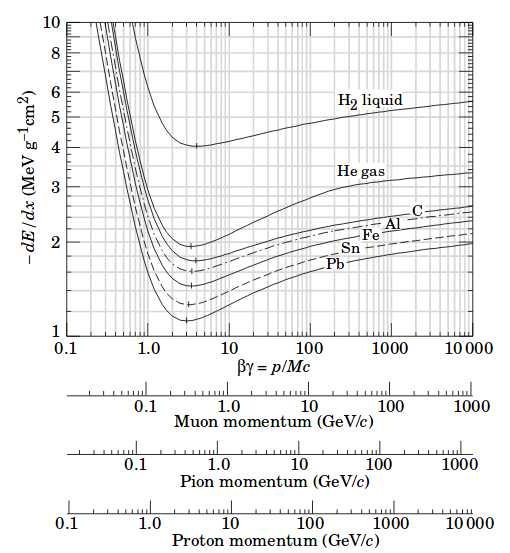
\includegraphics[width=0.50\textwidth]{images/PDGdEdX.png}
\caption{Mean energy loss in various materials over a range of particle momentums as produced in Reference \cite{PDG}.}
\label{fig:PDGEnergyLoss}
\end{figure}

Using the tables provided by the PDG for liquid argon (\cite{PDG-Argon}), we calculate the theoretical values for pions ($\pi$), muons ($\mu$), and protons ($p$) in the momentum range most relevant for LArIAT, shown in Figure \ref{fig:PDGEnergyLossArgon}.

\begin{figure}[htb]
\centering
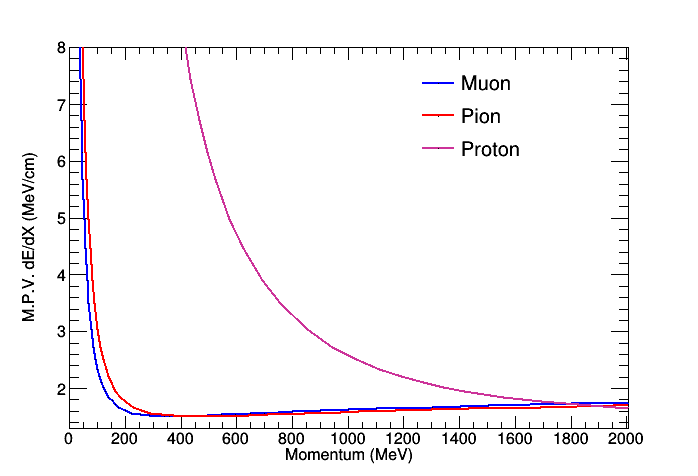
\includegraphics[width=0.50\textwidth]{images/dEdXvsMomentumTemplate}
\caption{Mean energy loss for pions, muons, and protons in liquid argon over the momentum range most relvant for LArIAT.}
\label{fig:PDGEnergyLossArgon}
\end{figure}

Using the predictions in Figure \ref{fig:PDGEnergyLossArgon}, allows us to tune the calorimetry constants used to convert the ADC to charge. The goal is to have the data and MC agree across the broad range of momentum. This tuning is done in addition to the wire-by-wire corrections (described in detail in \href{http://lartpc-docdb.fnal.gov:8080/cgi-bin/RetrieveFile?docid=1994&filename=investigation-uniformity-observed_v3.pdf&version=2}{doc-DB 1994}) and the usual lifetime corrections (described in detail in \href{http://lartpc-docdb.fnal.gov:8080/cgi-bin/ShowDocument?docid=1804}{docDB-1804}) which are used here and a more detailed treatment is left to their corresponding technical notes.

%%%%%%%%%%%%%%%%%%%%%%%%%%%%%%%%%%%%%%%%%%%%%%%%%%%%%%%%%%%
\subsection{Calibration Method Overview}\label{sec:MethodOverview}
%%%%%%%%%%%%%%%%%%%%%%%%%%%%%%%%%%%%%%%%%%%%%%%%%%%%%%%%%%%

In this section, we will describe the methodology we use to select our samples and tune the calorimetry constants. Details specific to any one sample will be described in Section  \ref{sec:EventSelection} and instead we will present the general method and how it is applied. 

The basic idea of this calibration technique is to utilize portion of a track within the LArTPC that has a well known momentum and particle species to measure the energy deposited per unit length (dE/dX) as recorded inside the TPC. Once a sample of particles dE/dX has been measured at various momentums, we then tune to calorimetry constants within the reconstruction software align these measured values to match the theoretical ones found in Figure \ref{fig:PDGEnergyLossArgon}.

Since various electronics changes and fixes to the PMT system were done between Run-I and Run-II, we derive calibration constants independently for both of these run periods. These calibration constants are the factors which convert the charge collected (dQ) to energy (dE). The details of how the calorimetry package works is beyond the scope of this note and is given in \href{http://lartpc-docdb.fnal.gov:8080/cgi-bin/ShowDocument?docid=2444}{docDB-2444}.

The calibration procedure follows the following basic steps:
\begin{itemize}

\item \textbf{Particle Identification in the beamline:}

We first select a sample of beamline events that correspond to either a sample of $\pi, \mu, e$ or protons. This is done by selecting based on the measured time-of-flight (TOF) vs momentum as measured in the wire chambers. We start by requiring the tracks reconstructed in the wire chamber satisfy the criteria known as a ``picky'' track, meaning the track reconstructed from the four wire chambers has a hit in each wire chamber. In these events, one and only one wire chamber track can be reconstructed per event. These tracks have a more accurate measure of the particle momentum than the ``high yield'' tracks which only require hits in three out of four of the wire chamber tracks and can have mulitple wire chamber tracks reconstructed per event. The ``high yield'' sample is used as a cross-check with more statistics once the calibration constants are found.

The wire chamber track is extrapolated to the front face of the LArTPC giving a $x, y$ position expected for the track in the TPC. A simple flat correction to the energy loss by the particle as it traverses the material between the last wire chamber and the front face of the LArTPC.

For the Monte Carlo, no such beamline identification is done and instead we use the data-driven Monte Carlo (DDMC), which constructs the momentum and angular distributions for the single particle MC, and launches particles from the position of the fourth wire chamber (WC4) towards the TPC. We utilize the Monte Carlo truth for the position and momentum of the Monte Carlo particles as they enter the TPC.

\item \textbf{Matching LArTPC tracks to the wire chamber tracks:}

For each track reconstructed inside the TPC, the most upstream trajectory point (smallest $z$ position) is found. For that point we have it's $x, y, z$ as well as the calculated $p_{x}, p_{y}, and p_{z}$ (which is used to calculate the tracks $\theta, \phi$. Using this as well as the wire chamber tracks extrapolated $x, y, \theta, \phi$ we then select the event if there is one and only one TPC track which matches the wire chamber track. The exact matching criteria is given in Section \ref{sec:EventSelection}.

We now have the initial momentum (corrected for energy loss due to the upstream material) of the TPC track which we can use for our calibration.

For the Monte Carlo, the ``wire chamber'' matching is done treating the true position of the MC particle as it enters the TPC as the ``wire chamber'' track. The rest of the matching proceeds just as before.

\item \textbf{dE/dX sampling:}



\end{itemize}